
\begin{columns}[t]
	\begin{column}{0.68\textwidth}
		\vspace{-0.1in}
		\begin{block} {\large Input to the learning process}
			\begin{columns}[T]
				\centering
				\begin{column}{0.59\textwidth}
					\begin{itemize}
						\item A regular set of points $\mathbb{X}_{local}$ in the vicinity of $x_0$ are collision checked to generate a binary 2D map $o_{local}$ indicating the presence of obstacles in the workspace.
						\item The heuristic $h(x)$ is also evaluated at each $x \in \mathbb{X}_{local}$, resulting in a 2D matrix $h_{local}$.
					\end{itemize}
				\end{column}
				\begin{column}{0.20\textwidth}
					\centering
					\begin{figure}
					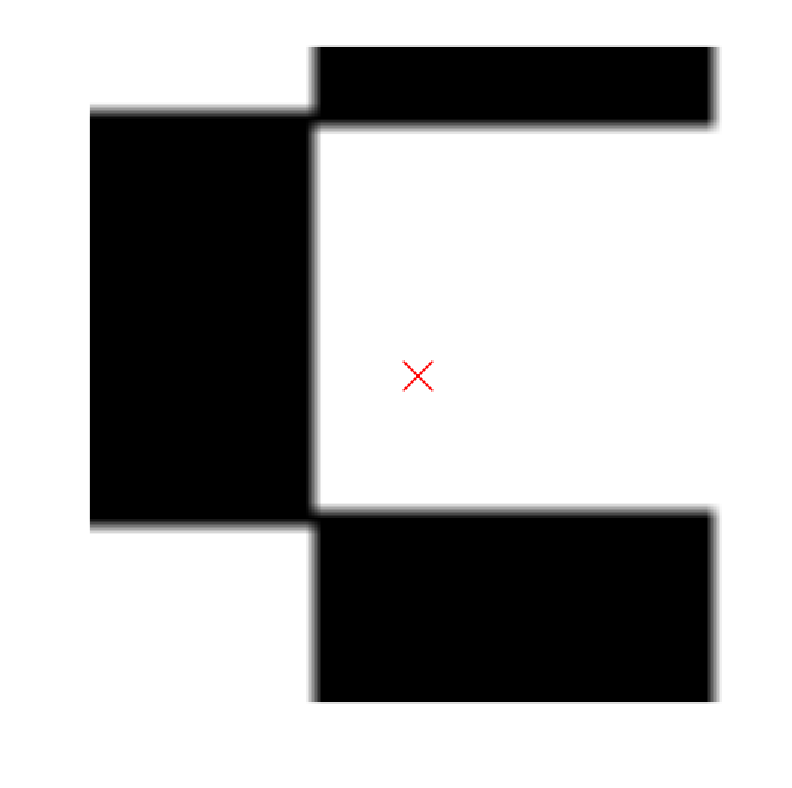
\includegraphics[width=0.5\columnwidth]{o_example}
					\caption{$o_{local}$} 
					\end{figure}
				\end{column}
				\begin{column}{0.20\textwidth}
					\centering
					\begin{figure}
					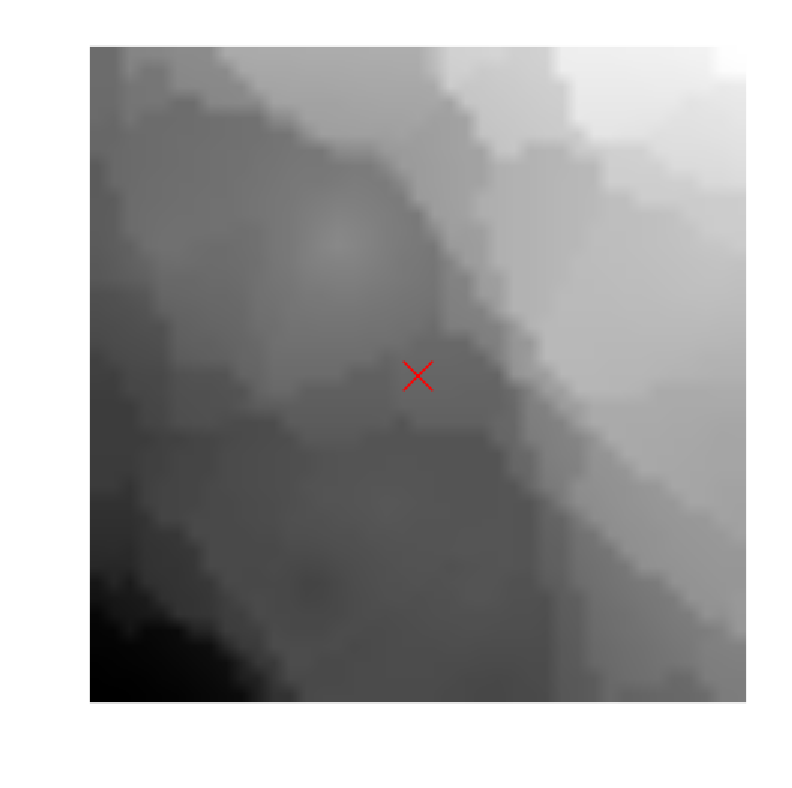
\includegraphics[width=0.5\columnwidth]{h_example}
					\caption{$h_{local}$} 
					\end{figure}
					\vspace{0.1in}
				\end{column}
			\end{columns}
		\end{block}
		\vspace{-0.1in}
		\begin{block}{\large Proposed architecture}
			\begin{itemize}
			\item Multi-layered neural networks $F_x, F_o, F_h$ act on the inputs to produce $x_0^*, o_{local}^*, h_{local}^*$. 
			\item An operator $M_0(x_0^*, o_{local}^*,h_{local}^*)$ produces feature vector  $x_f^0$.
			\item Exploitative control $u^0$ is obtained as $u^0 = F^0(x_f^0)$, where $F^0$ is also a neural network.
			\item Remaining $N$ exploratory controls are obtained as follows.
			\vspace{-.1in}
			\begin{align*}
				x_f^k &= M_k(x_f^0,U_{k-1}) \\
				u^{k} &= F^k(x_f^k) 
			\end{align*}
			\vspace{-.1in}
			where for all $k \geq 1$, $U_k = \{u^0,u^1,..,u^{k-1}\}$. For the exploitative control ($k=0$), $U_{k-1}$ is the empty set.
			\vspace{0.1in}
			\end{itemize}			
			\begin{figure}[h!]
				\centering
				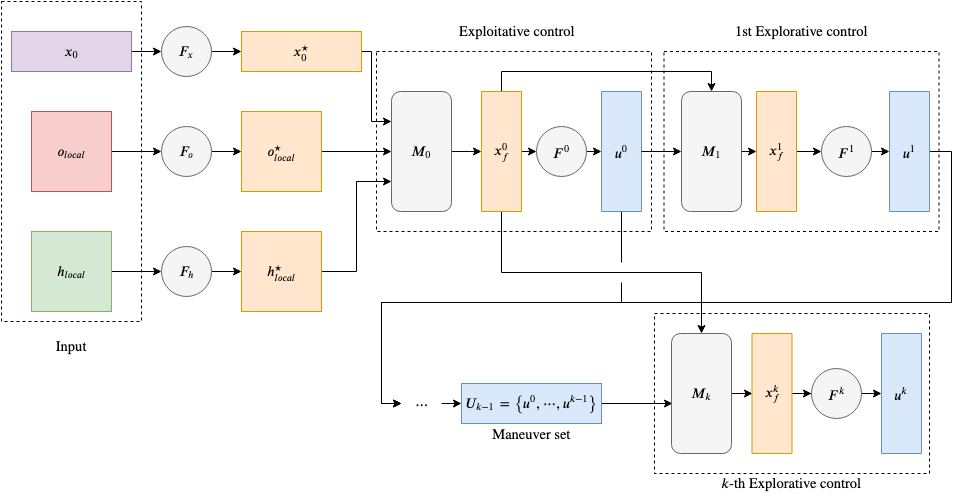
\includegraphics[scale=1.01]{cgraph}
				\vspace{-.1in}
				\caption{Computation graph of $U_k = \hat{f}(x_0,o_{local},h_{local})$. For $k=N, U_k = \hat{U} = \{u^0,\cdots,u^N\}$.\vspace{-.15in}}
				\label{fig:cgraph}
			\end{figure}
		\end{block}
	\end{column}
	\begin{column} {0.32\textwidth}
		\begin{block}{\large Evaluation}
		\begin{itemize}
			\item We consider a treaded vehicle with a 5 dim. state space (SE(2) augmented by steering angle and forward velocity) and 2 dim. control space (acceleration of left and right treads).
			\item For training, obstacles are randomly placed in a 2 dim. workspace so they cover one-third of the reachable workspace. 
			\item The DIRT planner $[1]$ is executed with the online curation procedure on multiple problem instances in such workspaces. 
			\item Euclidean distance to the goal in the workspace is used as the heuristic function. The cost is the duration of the solution trajectory.
			\item For each node $x_0$ the planner selects to propagate, the training process stores the  $o_{local}$ and $h_{local}$ maps, as well as a maneuver set $\hat{U}$ of size 5 curated from a set of 1000 randomly sampled maneuvers.
			\item Two networks - fully connected (\texttt{FC}) and convolutional (\texttt{Conv})
		\end{itemize}
		\centering
			\vspace{0.2in}
			\begin{columns}
				\centering
				\begin{column}{0.4\columnwidth} 
					\centering
					\begin{figure}
					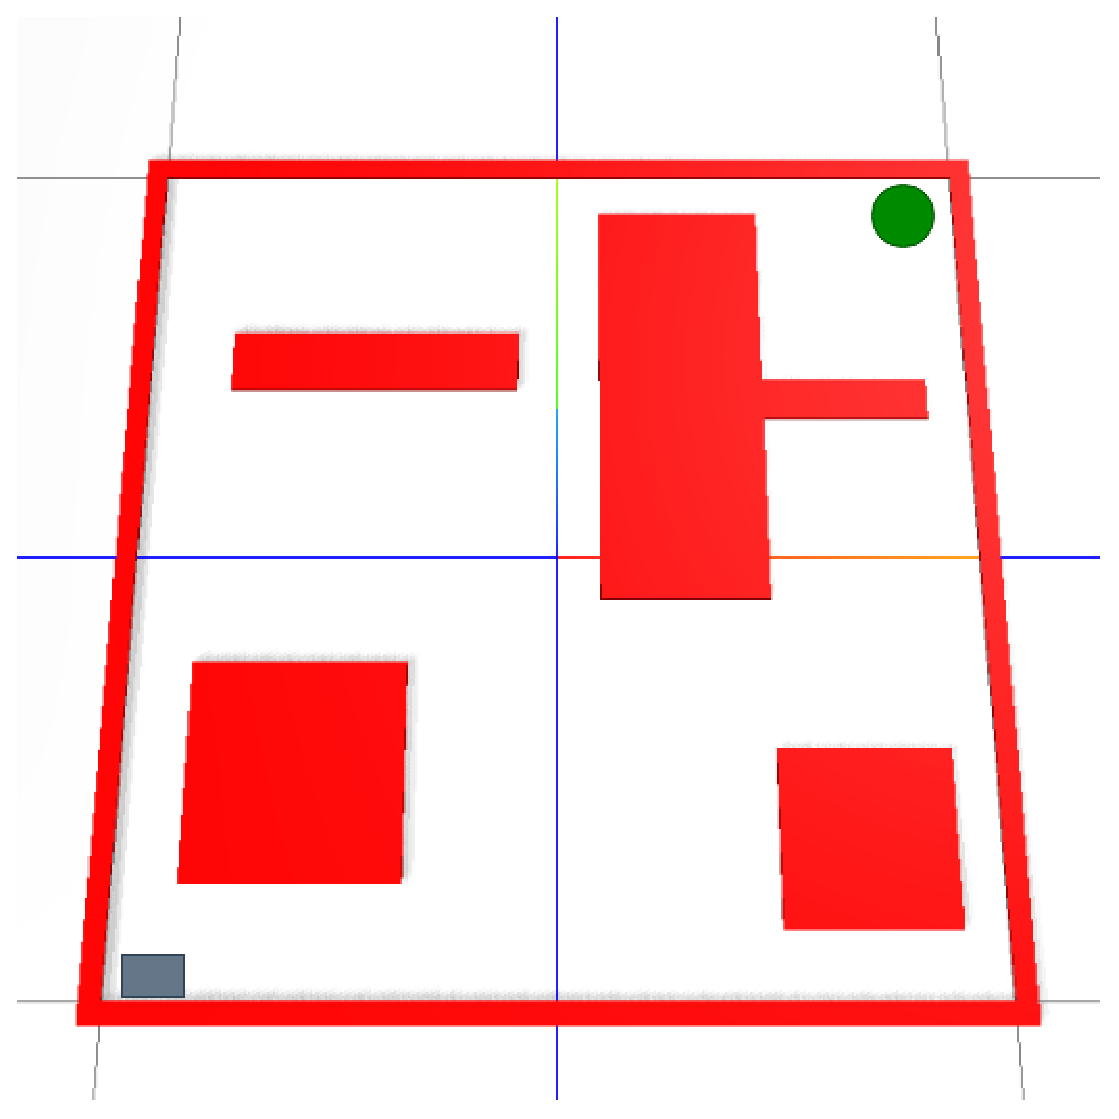
\includegraphics[width=\columnwidth]{iai}
					\caption{\texttt{Greedy}} 
					\end{figure}
				\end{column}
				\hfill
				\begin{column}{0.4\columnwidth} 
					\centering
					\begin{figure}
					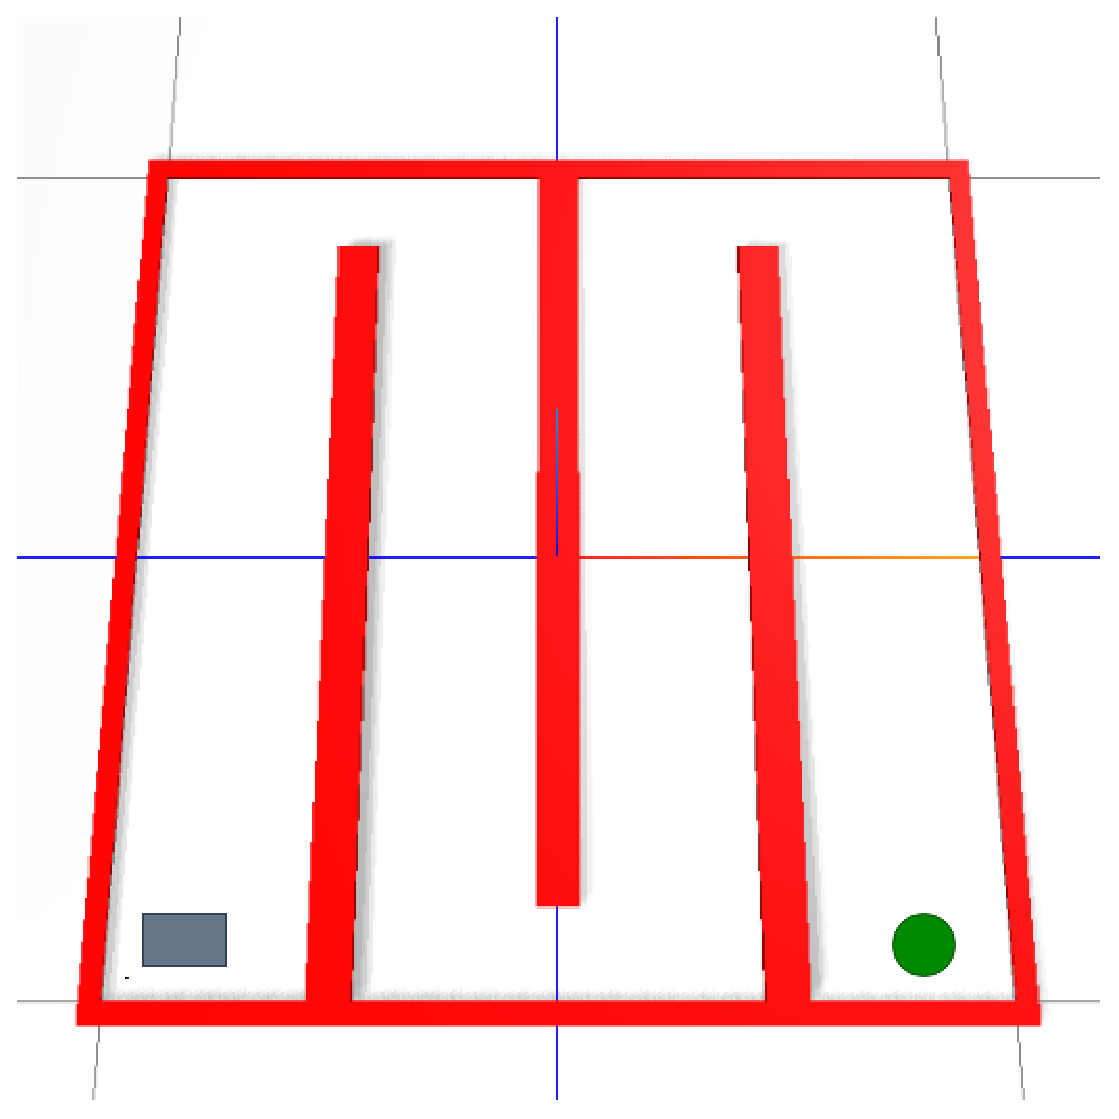
\includegraphics[width=\columnwidth]{flappy}
					\caption{\texttt{Explore}} 
					\end{figure}
				\end{column}
			\end{columns}
			\vspace{0.2in}
			Environments: The grey rectangle us the starting pose of the robot (facing right) and the green circle is the goal region. The robot must avoid the red obstacles.
			\vspace{0.1in}
		\end{block}
	\end{column}
\end{columns}



